\section[Magnetic impurities]{The Anderson and Kondo models}

%\texorpdfstring{Magnetic impurities in metals - \\ \null\hfill The Anderson and Kondo models}
%(page 183-> in pdf, 139-> in notes)

Imagine that we have a system defined by free, itinerant electrons, described by a conduction band with dispersion relation $\varepsilon_k$ and, for the sake of simplicity, assume that the one-particle density of state has a simple form as shown in Figure \ref{fig:dos}. The bandwidth of this system is $2D$, and the system has a Hamiltonian
\begin{equation}
	\label{eq:hamiltonian_free}
	\Ha_c = \sum_{k, \sigma}\varepsilon_k c_{k\sigma}^\dagger c_{k\sigma}.
\end{equation}

\begin{figure}[h]
	\centering
	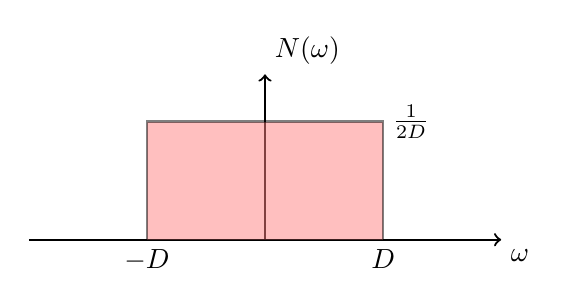
\begin{tikzpicture}[scale = 3]
	
	\draw[thick, ->] (0,1) -- (2,1);
	\draw[thick, ->] (1,1) -- (1,1.7);
	
	\draw[thick, draw = black,fill = red!50!white, opacity = 0.5] (0.5,1) rectangle (1.5,1.5);
	
	\node[anchor = north] at (0.5,1) {$-D$};
	\node[anchor = north] at (1.5,1) {$D$};
	\node[anchor = north west] at(2,1) {$\omega$};
	\node[anchor = south west] at (1,1.7){$N(\omega)$};
	\node[anchor = west] at (1.5, 1.5) {$\frac{1}{2D}$};
\end{tikzpicture}
	\caption{Density of states}
	\label{fig:dos}
\end{figure}

We will study the effect of including a magnetic impurity in the problem, where the magnetic impurity couples to the charged electrons, but is localized in space. First we consider the system with exactly one impurity. The Hamiltonian for this impurity is given by

\begin{equation}
\label{eq:hf}
	\Ha_f = E_0\sum_m f_m^\dagger f_m + U f_{\frac{1}{2}}^\dagger f_{-\frac{1}{2}}^\dagger f_{-\frac{1}{2}}f_{\frac{1}{2}},
\end{equation}

where $m$ are quantum numbers determining the z-component of the spin of the impurity. $(f_m, f_m^\dagger)$ are annihilation and creation operators for the impurity, in state $m$. $s = \frac{1}{2}: m = \pm 1$. $U$ is the Coulomb energy associated with double occupancy of the magnetic impurity. We will later assume that this is the largest energy in the system. The coupling between the charges and the localized impurity is given by
\begin{equation}
	\label{eq:interaction_term}
	\Ha_{cf}= \sum_{\vb k,\sigma,m}\left(V_{m\sigma}(\vb{k}) f_m^\dagger c_{\vb k\sigma}  + \text{h.c.}\right).
\end{equation}

In \eqref{eq:interaction_term}, $V_{m\sigma}(\vb k) $ is the matrix element transfering an electron from the impurity to the conduction band, or opposite. 
The total Hamiltonian is
\begin{equation}
	\Ha = \Ha_c + \Ha_f + \Ha_{cf}.
\end{equation}
$\Ha$ is often called the Anderson model. This model is the fundament for our understanding of heavy fermion systems. We will now use the techniques to study the effects of including a magnetic impurity in the conduction band. 
One important effect of magnetic impurities is that a metal will exhibit a minima in resistivity (see Figure \ref{fig:resistivity}).
\begin{figure}
	\centering
	\begin{tikzpicture}
    \begin{axis}[
        xmin = 0, xmax = 2,
        ymin = 0,% ymax = 1,
        axis lines = center,
        axis on top =true,
        domain = 0.1:1.6,
        %restrict y to domain=0:1,
        ylabel = $\rho(T)$,
        y label style={anchor=east},
        xlabel = $T$,
        xtick ={1},
        xticklabels={$T_K$},
        ytick style={draw=none},
        yticklabels={,,},
        samples = 100,
        %ticks = none
        ]
        
        \addplot[mark = none, draw = red!50!white, ultra thick]{1 -5*ln(x) + x^5};
        
        %\addplot[mark = none, draw = red!50!white, dashed]{1 -5*ln(x)};
        %\addplot[mark = none, draw = red!50!white, dashed]{x^5};
        
    	%\draw [thick] (axis cs:1.25,0)-- (axis cs:1.25,0.21);
    
        \node at (axis cs:0.6,5.5) {\footnotesize $\sim\ln T$};
        \node at (axis cs:1.25,6) {\footnotesize $T^5\sim $};
       	%\node[anchor = south] at (axis cs:1, 0) {$T_K = $ Kondo temperature};
        %\draw[->] (axis cs:3, 0.35) --(axis cs:4, 0.35) ;
    \end{axis}
\end{tikzpicture}
	\caption{Resistivity}
	\label{fig:resistivity}
\end{figure}
$T_K$ is only a couple of Kelvin, but the Fermi-energy is of order $10^4\mathrm{K}$. How can an energy scale this small arise when the basis is that the relevant energy scale is $\varepsilon_F \sim 10^4\mathrm{K}$? If magnetic impurities are excluded, the resistivity is uniformly decreasing. Jun Kondo found that $\rho(T) \sim -\ln T$ diverges in perturbation theory at low temperatures\footnote{Progress of Theoretical Physics, Vol. 32, No. 1, pp. 37-49}. A new problem then arises; how can we give a consistent description of low temperaturre physics, $T<<T_K$, in systems with a minima in resistivity? This problem is often referred to as the ``Kondo problem''. 

What we will do, is to see how the energy scale $T_K$, The Kondo temperature, arises, as well as to give a consistent description of the lowæ-temperature physics in metals doped with magnetic impurities, in a saddle point approxiimation.
Typical materials described by these theories are metals like aluminium and gold, doped with other rare materials. These materials are then the magnetic impurities in the problem. Rare materials: Lanthanides and actinides. Most studied: Cerium (Lanthanide) and Uranium (actinide). In the lanthanides the valence electrons are in the 4f-shell, and in actinides they are in the 5f-shell (hence $f_m^\dagger, f_m)$). Regularly studied materials are $\mathrm{CeAl_2}$ (lanthanide) and $\mathrm{UPt_3}$ (Actinide). $\mathrm{UPt_3}$ is a very odd superconductor with $T_C \sim 1\mathrm{mK}$ and a very complicated order parameter.  

Let us simplify the Anderson model;

\textbf{i)}: $U = \infty$.

Doubly occupancy of the magnetic impurities are not allowed. If there already exist a spin on the lattice site of the impurity, a conducting electron can not enter this localized orbital.

\textbf{ii)}: We assume that the coupling between $f$- and $c$-electrons are such that $m = \sigma$,  i.e. 
\begin{equation}
	V_{m\sigma}(k) =\delta_{m\sigma}V(k), 
\end{equation}
and that $V(k)$ is $k$-independent (completely localized coupling)
\begin{equation}
	V_{m\sigma}(k) = V\delta_{m\sigma}
\end{equation}
which implies
\begin{equation}
	\Ha_{cf} = V\sum_{\sigma k}\left(f_\sigma^\dagger c_{k\sigma} + h.c.\right).
\end{equation}

Thus, we have the model 
\begin{align}
	\begin{split}
	\Ha &= E_0\sum_{\sigma}f_\sigma^\dagger f_\sigma + \sum_{k,\sigma}\varepsilon_k c_{k\sigma}^\dagger c_{ck}^\dagger \\
	&= V\sum_{k,\sigma}\left[f_{\sigma}^\dagger c_{k\sigma} + h.c. \right],
	\end{split}
\end{align}

with \(\sum_mf_m^\dagger f_m \leq 1 \). It is the restiriction on the occupation number on the impurities that makes this a hard problem.

For later reference, we first solve the problem with $U = 0$.
\subsection{$U = 0$}

\begin{equation}
\Z = \int \D c^\dagger \D c\D f^\dagger \D f\e^{\Sa}
\end{equation}
\begin{equation}
\Sa = -\int\left(\sum_{k,\sigma}c_{k\sigma}^\dagger\pdv{c_{k\sigma}}{\tau} + \sum_mf_m^\dagger \pdv{f_m}{\tau} + \Ha \right)\dd{\tau}
\end{equation}

\begin{align}
\begin{split}
\Sa = &- \int_0^\beta\sum_{k,\sigma}c_{k\sigma}^\dagger\left(\partial_\tau + \varepsilon_k\right)c_{k\sigma} \dd{\tau} \\
&-\int_0^\beta\sum_\sigma f_\sigma^\dagger\left(\partial_\tau + E_0\right)f_\sigma \dd{\tau}\\
&-\int_0^\beta V\sum_{k, \sigma}\left(f_\sigma^\dagger c_{k\sigma} + h.c.\right)\dd{\tau}
\end{split}
\end{align}
\(\Z\) can be computed exactly by a linear shift og the fermion operators \((c_{k\sigma}, c_{k\sigma}^\dagger)\). Introduce \(\Gre^{-1}= \partial_\tau + \varepsilon_k\). Consider now the quantity
\begin{align}
\label{eq:temp_derivation}
	&\sum_{k, \sigma}\left[c_{k\sigma}^\dagger \Gre^{-1}c_{k\sigma}+ Vf_{\sigma}^\dagger c_{k\sigma} + Vc_{k\sigma}^\dagger f_\sigma\right] \nonumber\\
	&= \sum_{k\sigma}\left(c_{k\sigma}^\dagger + Vf_\sigma^\dagger \Gre\right)\Gre^{-1}\left(c_{k\sigma} + V\Gre f_\sigma\right) -\sum_{k,\sigma}V^2f_\sigma^\dagger \Gre f_\sigma \nonumber\\
	&=\sum_{k\sigma}\tilde{c}_{k\sigma}^\dagger \Gre^{-1}\tilde{c}_{k\sigma} - \sum_\sigma f_\sigma^\dagger\left(\sum_k V^2\Gre\right)f_\sigma.
\end{align}
Inserting \eqref{eq:temp_derivation} into the action, we get
\begin{equation}
\label{eq:action_magnetic}
	S =-\sum_{k,\sigma}\tilde{c}_{k\sigma}^\dagger \Gre^{-1}\tilde{c}_{k\sigma}-\sum_\sigma f_\sigma^\dagger\left(\partial_\tau + E_0 - V^2\sum_k\frac{1}{\partial_\tau + \varepsilon_k}\right)f_\sigma.
\end{equation}
As we can see in \eqref{eq:action_magnetic}, the action is quadratic in the $c$- and $f$- sectors.

\begin{equation}
	\Z = \int\D\tilde{c}^\dagger\D\tilde{c}\D f^\dagger \D f\, \e^{\Sa}= \Z_c\cdot\Z_f,
\end{equation}
where 
\begin{align}
	\Z_c &= \e^{\Tr\ln \left(\Gre^{-1}\right)} & \Z_f&= \e^{\Tr\ln\left(\mathcal{G}_f^{-1}\right)}\\
	\label{eq:fermi_propagator}
	\Gre^{-1} &= \partial_\tau + \varepsilon_k &
	\mathcal{G}_f^{-1} &= \partial_\tau + E_0 -V^2\sum_k \frac{1}{\partial_\tau + \varepsilon_k}.
\end{align}

$\Z_c$ is the partition function for free electron gas, and $\Z_f$ is the partition function for the impurities, coupled to a free electron gas.

we have already considered
\begin{equation}
\label{eq:free_energy_non_interacting}
	\Tr\ln\Gre^{-1} = \sum_{k,\sigma}\ln\left(1 + \e^{-\beta\varepsilon_k}\right).
\end{equation}
\eqref{eq:free_energy_non_interacting} is the free energy for non-interacting electron gas, as we have seen earlier (see the derivation of \eqref{eq:partition_free_electron}).

\begin{equation}
\label{eq:trace_impurities}
	\Tr\ln\left(\mathcal{G}_f^{-1}\right) = \sum_\sigma\sum_{\omega_n}\ln\left(-i\omega_n + E_0 +V^2\sum_k \frac{1}{i\omega_n - \varepsilon_k}\right)
\end{equation}

Consider now the last $k$-summation in \eqref{eq:trace_impurities}.
\begin{align}
\label{eq:k_sum}
\begin{split}
	\sum_k\frac{1}{i\omega_n - \varepsilon_k} &= \frac{1}{2D}\int_{-D}^D\dd{\varepsilon}\frac{1}{i\omega_n - \varepsilon} \\
	&= \frac{1}{2D}\ln\left(\frac{D+i\omega_n}{-D + i\omega_n}\right)\\
	&=-\frac{1}{2D}\ln\left(\frac{\omega_n+iD}{\omega_n-iD}\right)
\end{split}
\end{align}
This is evaluated as
\begin{equation}
	\ln\left(\frac{z}{z^*}\right) = \ln\left(\frac{|z|e^{i\varphi}}{|z|\e^{-i\varphi}}\right) = 2i\varphi.
\end{equation}
Here, $\varphi = \tan[-1](\frac{D}{\omega_n}) \simeq \frac{\pi}{2}\mathrm{sgn}(\omega_n)$ as $T\rightarrow 0$.
This implies that we can write the $k$-sum in \eqref{eq:k_sum} as
\begin{align}
	\sum_k\frac{1}{i\omega_n - \varepsilon_k} &\simeq -i\frac{\pi\cdot 2}{2\cdot 2D}\mathrm{sgn}(\omega_n)\\
	&= -i\pi\rho_0\mathrm{sgn}(\omega_n)
\end{align}
where we introduced $\rho_0 = \flatfrac{1}{2D}$. Define $\Delta_0 \equiv \pi\rho_0 V^2$. Going back to \eqref{eq:trace_impurities}, we now have
\begin{equation}
	\sum_k\frac{1}{i\omega_n - \varepsilon_k} = \sum_\sigma\sum_{\omega_n}\ln\left(-i\omega + E_0 - i\Delta_0 \mathrm{sgn}(\omega_n)\right).
\end{equation}
Following the same methods as we have seen earlier, we have
\begin{align}
	\sum_{\omega_n}\dots &= \frac{-\beta}{2\pi i}\oint\dd{z}f(z)\ln(-z+E_0-i\Delta_0\mathrm{sgn}(\Im{z}))\nonumber\\
	&= -\frac{\beta}{2\pi i }\int_{-D}^{D}\dd{\varepsilon}f(\varepsilon)\left[\ln(-\varepsilon + E_0- i\Delta_0) - \ln(-\varepsilon + E_0 + i\Delta_0)\right] \nonumber\\
	\label{eq:action_derivation}
	&= \frac{\beta}{\pi}\int_{-D}^D\dd{\varepsilon}f(\varepsilon)\tan[-1](\frac{\Delta_0}{E_0 - \varepsilon}).
\end{align}
Thus, after the spin-summation, our total action is
\begin{equation}
\label{eq:action_impurities}
	\Sa = -2\sum_k\ln\left(1 + \e^{-\beta\varepsilon_k}\right) + \frac{2\beta}{\pi}\int_{-D}^D\dd{\varepsilon}f(\varepsilon)\tan[-1](\frac{\Delta_0}{E_0 - \varepsilon}).
\end{equation}
$\Sa$ describes a free electron gas, plus a scattering resonance at the energy $E_0$ caused by the coupling between  $f$- and $c$-electrons. Notice that if $|E_0| >> D$ ,the second term in \eqref{eq:action_impurities} can be neglected. The impurities are far from the conduction band, and does not matter. When $U = \infty$, this will drastically change this result, as we shall now see.

NB! The Green's functions:
\begin{align*}
	-\ev{ff^\dagger} &= -\left(\partial_\tau + E_0 - V^2 \sum_k\frac{1}{\partial_\tau + \varepsilon_k}\right)^{-1}\\
	&\rightarrow \left(i\omega_n-E_0 + V^2\sum_k \frac{1}{i\omega_n - \varepsilon_k}\right)^{-1} \\
	-\ev{\tilde{c}\tilde{c}^\dagger} &= -\frac{1}{\partial_\tau + \varepsilon_k} \\
	&\rightarrow \frac{1}{i\omega_n-\varepsilon_k},
\end{align*}
but the $\tilde{c}$-``electrons'' are \underline{not} physical electrons. We defined them as $\tilde{c} = c+V\Gre f_\sigma \Rightarrow c = \tilde{c} - V\Gre f_\sigma$.
Then, the conducting-electron-propagator is modified;
\begin{align*}
	-\ev{cc^\dagger} &= -\left[\ev{(\tilde{c}-V\Gre f_\sigma)(\tilde{c}^\dagger - V\Gre f_\sigma^\dagger)}\right]\\
	&= -\Gre + V\Gre\ev{\tilde{c}f^\dagger} + V\Gre\ev{f\tilde{c}^\dagger} - V^2\Gre\ev{ff^\dagger}\Gre
\end{align*}

The propagator for the conducting electrons is then
\begin{equation}
	\mathcal{G}(\partial_\tau, \varepsilon_k) = -\left[\Gre(\partial_\tau, \varepsilon_k) + V^2\Gre(\partial_\tau, \varepsilon_k)\mathcal{G}_f(\partial_\tau)\Gre(\partial_\tau, \varepsilon_k)\right]
\end{equation}
\subsection{$U = \infty$}
Remember that $U$ is the energy of the Coloumb interaction from double occupancy of the impurities defined in \eqref{eq:hf}.
\begin{equation}
	\Ha = E_0\sum_\sigma F_\sigma^\dagger F_\sigma + \sum_{k,\sigma}\varepsilon_k c_{k\sigma}^\dagger c_{k\sigma} + V\sum_{k,\sigma}\left(F_\sigma^\dagger c_{k\sigma} + c_{k\sigma}^\dagger F_\sigma\right)
\end{equation}
Our constraint reads
\begin{equation}
\sum_m F_m^\dagger F_m \le 1,
\end{equation}
i.e. we have \underline{no} double occupancy. As we did for the Hubbard model at $U = \infty$, wee introduce $b$-bosons.
\begin{align*}
	F_m^\dagger &= f_m^\dagger b \\
	F_m &= f_mb^\dagger\\
	\sum_m &f_m^\dagger f_m + b^\dagger b = 1
\end{align*}
$F_m, F_m^\dagger$ are Hubbard operators, and does not satisfy simple commutation relations. When this restriction is satisfied, we have
\begin{equation}
	\Ha = E_0\sum_m f_m^\dagger f_m + \sum_{k,\sigma}\varepsilon_k c_{k\sigma}^\dagger c_{k\sigma} + V\sum_{k,\sigma}\left(f_\sigma^\dagger bc_{k\sigma} + c_{k\sigma}^\dagger b^\dagger f_\sigma\right)
\end{equation}
with the restriction 
\begin{equation}
	\sum_m f_m^\dagger f_m + b^\dagger b = 1 \equiv Q.
\end{equation}
As we did for  $U=\infty$ Hubbard:
\begin{align}
	\Z &= \int\mathcal{D}c^\dagger\mathcal{D}c\mathcal{D}f^\dagger\mathcal{D}f\mathcal{D}b^\dagger\mathcal{D}b\,\e^{\Sa}\delta_{Q,1} \\
	\begin{split}
	\Sa &= -\sum_m\int_0^\beta \dd{\tau} f_m^\dagger\left(\partial_\tau + E_0\right)f_m - \sum_{k,\sigma}\int_0^\beta \dd{\tau} c_{k\sigma}\left(\partial_\tau + \varepsilon_k\right) c_{k\sigma}) \\
	&\quad -\int_0^\beta \dd{\tau}b^\dagger\partial_\tau b - V\sum_{k, \sigma}\int_0^\beta \dd{\tau}\left(c_{k\sigma}^\dagger b^\dagger f_\sigma + f_\sigma^\dagger b c_{k\sigma}\right).
	\end{split}
\end{align}
Again, we use Abrikosov's trick, that for each value of $\tau$ use that
\begin{align}
	\delta_{Q,1} &= \int_{-\pi}^\pi \frac{\dd{\lambda}}{2\pi}\e^{-i\lambda(Q-1)} \\
	\Rightarrow \Z &= \int_{-\pi}^\pi \frac{\dd{\lambda}}{2\pi}\int\mathcal{D}c^\dagger\mathcal{D}c\mathcal{D}f^\dagger\mathcal{D}f\mathcal{D}b^\dagger\mathcal{D}b\,\e^{\tilde{\Sa}} \\
	\begin{split}
		\tilde{\Sa} &= -\sum_m\int_0^\beta \dd{\tau} f_m^\dagger\left(\partial_\tau + E_0 + i\lambda\right)f_m - \sum_{k,\sigma}\int_0^\beta \dd{\tau} c_{k\sigma}\left(\partial_\tau + \varepsilon_k\right) c_{k\sigma}) \\
		&\quad -\int_0^\beta \dd{\tau}b^\dagger\left(\partial_\tau + i\lambda\right) b - V\sum_{k, \sigma}\int_0^\beta \dd{\tau}\left(c_{k\sigma}^\dagger b^\dagger f_\sigma + f_\sigma^\dagger b c_{k\sigma}\right) + i\int_{0}^\beta\dd{\tau}\lambda  
	\end{split}
\end{align}
Again we introduce $\Gre = \partial_\tau + \varepsilon_k$, and make a shift of the $c$-fields:
\begin{align*}
	\sum_{k\sigma}&\left[c_{k\sigma}^\dagger \Gre^{-1}c_{k\sigma} + V\left(c_{k\sigma}^\dagger b^\dagger f_\sigma + f_\sigma^\dagger bc_{k\sigma}\right)\right]\\
	&=\sum_{k,\sigma}\underbrace{\left(c_{k\sigma}^\dagger + Vf_{\sigma}^\dagger b\Gre\right)}_{\tilde{c}^\dagger}\Gre^{-1}\left(c_{k\sigma} + V\Gre b^\dagger f_\sigma\right) \\
	&\quad - V^2\sum_\sigma f_\sigma^\dagger b\left(\sum_k\Gre\right)b^\dagger f_\sigma
\end{align*}
Now, do the functional integrals $\int\mathcal{D}\tilde{c}^\dagger\mathcal{D}\tilde{c}$ such that $\Z = \Z_0\cdot\tilde{\Z}$ with 
\begin{equation*}
\Z_0 = \e^{\Tr\ln\Gre^{-1}}
\end{equation*}
and
\begin{equation*}
	\tilde{\Z} = \int_{-\pi}^\pi \frac{\dd{\lambda}}{2\pi}\int\mathcal{D}f^\dagger\mathcal{D}f\mathcal{D}b^\dagger\mathcal{D}b\,\e^{\Sa_{\text{eff}}},
\end{equation*}
where 
\begin{align*}
\Sa_{\text{eff}} = \int_0^\beta\dd{\tau}[-b^\dagger\left(\partial_\tau + i\lambda\right)b &- \sum_m f_m^\dagger\left(\partial_\tau + E_0 + i\lambda\right)f_m\\
&+ \sum_m f_m^\dagger V^2 b\left(\sum_k\Gre\right)b^\dagger f_m \\
&+i\lambda]
\end{align*}
We can now do the $\int\mathcal{D}f^\dagger\mathcal{D}f$-integration:
\begin{equation}
	\tilde{\Z} = \int_{-\pi}^\pi\frac{\dd{\lambda}}{2\pi}\int\mathcal{D}b^\dagger\mathcal{D}b\,\e^{\tilde{\Sa}_{\text{eff}}[b^\dagger, b, \lambda]}.
\end{equation}
The theory is now bosonized, with
\begin{align}
\tilde{\Sa}_{\text{eff}}[b^\dagger, b, \lambda] &= -\int_0^\beta \dd{\tau}\left(b^\dagger\left(\partial_\tau + i\lambda\right)b + i\lambda\right) + \Tr\ln(\mathcal{G}_f^{-1}[b^\dagger, b, \lambda]) \\
\mathcal{G}_f^{-1} &= \partial_\tau + E_0 + i\lambda-V^2b^\dagger\left(\sum_k\frac{1}{\partial_\tau + \varepsilon_k}\right)b
\end{align}
Remembering the results \eqref{eq:fermi_propagator} for $U=0$, we see that $U=\infty$ has two effects:
\begin{enumerate}[i]
	\item Shift of $E_0$
	\item Renormalized hybridisation
\end{enumerate} 
Again, the resulting effective action is to complicated to be calculated exactly. Let us therefore introduce a saddle point approximation by
\begin{align*}
b(\tau)&= b\\
i\lambda &=\lambda.
\end{align*}

\begin{align}
	\tilde{\Sa}_{\text{eff}} &= -\beta\lambda(b^2-1) + \Tr\ln\left(\partial_\tau + E_0 + \lambda-V^2b^2\sum_k\Gre\right)\nonumber \\
	&=-\beta\lambda(b^2-1) + \sum_\sigma\sum_{\omega_n}\ln\left(-i\omega_n + \varepsilon_f + s_0^2\sum_k\frac{1}{i\omega_n-\varepsilon_k}\right)\nonumber \\
	&= -\beta\lambda(b^2-1) + 2\sum_{\omega_n}\ln\left(-\omega_n + \varepsilon_f -i\Delta\mathrm{sgn}(\omega_n)\right)\nonumber \\
	\label{eq:effective_action}
	&= -\beta\lambda(b^2-1) + 2\beta\int_{-D}^D \frac{\dd{\varepsilon}}{\pi}f(\varepsilon)\tan[-1](\frac{\Delta}{\varepsilon_f - \varepsilon}),
\end{align}
where we introduced $s_0 \equiv bV, \Delta \equiv \pi\rho_0s_0^2$ and followed the same derivation as \eqref{eq:action_derivation} with the appropriate changes.
If we compare \eqref{eq:effective_action} with the effective action from the $U = 0$ -case,
\begin{equation}
	\Sa_{\text{eff}, U=0}  = 2\beta\int_{-D}^D\frac{\dd{\varepsilon}}{\pi}f(\varepsilon)\tan[-1](\frac{\Delta_0}{E_0 - \varepsilon}),
\end{equation}
we have for $U=\infty$ a shift in the scattering resonance at $\varepsilon_f = E_0 + \lambda$. As we will now see, $\varepsilon_f$ is ``nailed'' to the Fermi-level, such that even if $E_0$ is far outside the conduction band, $\varepsilon_f$ is practically on the Fermi level. Thus, impurities always affect the physics at the Fermi level. This permanent nailing is the origin of the Kondo-effect and heavy-fermion behaviour. \textbf{This is thus a correlation effect.}
We will now minimize the effective action with respect to $b^2$ and $\lambda$. 
$\varepsilon_f = E_0 + \lambda \Rightarrow \lambda = \varepsilon_f - E_0$, and $s_0 = bV \rightarrow b^2 = \flatfrac{s_0^2}(V^2)$. Then

\begin{align}
	\tilde{\Sa}_{\text{eff}} &=  -\beta\left(\varepsilon_f - E_0\right)\left(\frac{s_0^2}{V^2} - 1\right) \\
	&+ 2\beta\int_{-D}^D\frac{\dd{\varepsilon}}{\pi}f(\varepsilon)\tan[-1](\frac{\Delta}{\varepsilon_f-\varepsilon})
\end{align}

\begin{align}
	\label{eq:self_cons1}
	\pdv{\tilde{\Sa}_{\text{eff}}}{\varepsilon_f} &= 0 \\
	\label{eq:self_cons2}
	\pdv{\tilde{\Sa_{\text{eff}}}}{s_0}&= 0
\end{align}
Eqs. \eqref{eq:self_cons1},\eqref{eq:self_cons2} are self consistent equations for deciding $\varepsilon_f, s_0$. 

Notice also that for $T=0$, the effective action is well defined. The method therefore gives a well defined description of the low-$T$ physics.
Consider the $T = 0$ case:
\begin{align}
	\tilde{\Sa}_{\text{eff}} &= -\beta\left(\varepsilon_f - E_0\right)\left(\frac{s_0^2}{V^2} -1\right) \\
	&+ 2\beta\int_{-D}^{0}\frac{\dd{\varepsilon}}{\pi}\tan[-1](\frac{\Delta}{\varepsilon_f-\varepsilon}) \\
	&\tan[-1](x) = \frac{-i}{2}\ln\left(\frac{1+ix}{1-ix}\right)
\end{align}
And the quantity 
\begin{align*}
	\int_{-D}^0\frac{\dd{\varepsilon}}{\pi}\tan[-1](\frac{\Delta}{\varepsilon_f-\varepsilon}) &= \int_{0}^D\frac{\dd{\varepsilon}}{\pi}\tan[-1](\frac{\Delta}{\varepsilon_f + \varepsilon}) \\
	&= \int_{\varepsilon_f}^{D + \varepsilon_f}\frac{\dx}{\pi}\tan[-1](\frac{\Delta}{x}) \\
	&= \frac{1}{\pi}\bigg|_{\varepsilon_f}^{D + \varepsilon_f}x\tan[-1](\frac{\Delta}{x}) - \frac{1}{\pi}\int_{\varepsilon_f}^{D + \varepsilon_f}\dx \frac{x}{1 +\frac{\Delta^2}{x^2}}\left(\frac{-\Delta}{x^2}\right) \\
	&= \frac{1}{\pi}\left[\left(D+\varepsilon_f\right)\tan[-1](\frac{\Delta}{D+\varepsilon_f}) - \varepsilon_f\tan[-1](\frac{\Delta}{\varepsilon_f})\right] \\
	&\qquad+ \frac{\Delta}{2\pi}\ln\left(\frac{\left(D+\varepsilon_f\right)^2 + \Delta^2}{\varepsilon_f^2 + \Delta^2}\right) \\
	&\stackrel{D>>(\Delta, \varepsilon_f)}{\simeq} \frac{-\varepsilon_f}{\pi}\tan[-1](\frac{\Delta}{\varepsilon_f}) - \frac{\Delta}{2\pi}\ln\left(\frac{\varepsilon_f^2 + \Delta^2}{D^2}\right) \\
	&\qquad +\frac{D+\varepsilon_f}{\pi}\tan[-1](\frac{\Delta}{D+\varepsilon_f})
\end{align*}
Now $\varepsilon_f + D >>(\Delta, \varepsilon_f) \Rightarrow \tan[-1](\flatfrac{\Delta}(D+\varepsilon)) \simeq \flatfrac{\Delta}(D+\varepsilon_f)$ which implies 
\begin{align*}
	&\frac{\Delta}{\pi} - \frac{\varepsilon_f}{\pi}\tan[-1](\flatfrac{\Delta}(\varepsilon_f)) - \frac{\Delta}{2\pi}\ln\left(\frac{\varepsilon_f^2 + \Delta^2}{D^2}\right) \\
	&\simeq \int_{-D}^0\dd{\varepsilon}\tan[-1](\frac{\Delta}{\varepsilon_f - \varepsilon})
\end{align*}

\begin{align}
\begin{split}
	\tilde{\Sa}_{\text{eff}}&= -\beta(\varepsilon_f -E_0)\left(\frac{\Delta}{\Delta_0}-1\right) \\
	\quad &+2\beta\left(\frac{\Delta}{\pi} - \frac{\varepsilon_f}{\pi}\tan[-1](\frac{\Delta}{\varepsilon_f}) - \frac{\Delta}{2\pi}\ln\left(\frac{\varepsilon_f^2 + \Delta^2}{D^2}\right)\right) =-\beta\tilde{U}_\text{eff},
\end{split}
\end{align}
at $T = 0$. $\flatfrac{s_0^2}{V^2} = \flatfrac{\Delta}{\Delta_0}$ with $\Delta = \pi\rho_0 s_0^2, \Delta = \pi\rho_0 V^2$.
The equations to evaluate are
\begin{align*}
	\pdv{\tilde{U}_\text{eff}}{\Delta} = 0 &&
	\pdv{\tilde{U}_\text{eff}}{\varepsilon_f} = 0
\end{align*}
\begin{align*}
\pdv{\tilde{U}_\text{eff}}{\Delta} &= 0 = \frac{1}{\Delta_0}(\varepsilon_f - E_0) - \frac{2}{\pi} + \frac{2\varepsilon_f}{\pi}\frac{1}{1+\frac{\Delta^2}{\varepsilon_f^2}}\frac{1}{\varepsilon_f} \\
&\quad+ \frac{1}{\pi}\ln\left(\frac{\varepsilon_f^2 +\Delta^2}{D^2}\right) + \frac{\Delta}{\pi}\frac{2\Delta}{\varepsilon_f^2 + \Delta^2} \\
&= \frac{1}{\Delta_0}(\varepsilon_f-E_0)-\frac{2}{\pi} + \frac{2}{\pi}\left(\frac{\varepsilon_f^2 + \Delta^2}{\varepsilon_f^2+\Delta^2}\right) + \frac{1}{\pi}\ln\left(\frac{\varepsilon_f^2 +\Delta^2}{D^2}\right) = 0  \\
\Rightarrow &\frac{\Delta_0}{\pi}\ln\left(\frac{\varepsilon_f^2 + \Delta^2}{D^2}\right) = E_0 - \varepsilon_f \\
\pdv{\tilde{\Sa}_{\text{eff}}}{\varepsilon_f} &= 0 = \frac{\Delta}{\Delta_0} -1 +\frac{2}{\pi}\tan[-1](\frac{\Delta}{\varepsilon_f}) \\
\Rightarrow &
\frac{2}{\pi}\tan[-1](\frac{\Delta}{\varepsilon_f}) = 1-\frac{\Delta}{\Delta_0} \equiv \sum_m\langle f_m^\dagger f_m\rangle = n_f
\end{align*}

\begin{align*}
\pdv{\tilde{\Sa}_{\text{eff}}}{\varepsilon_f} &= 0 \\
&=\frac{\Delta}{\Delta_0} - 1+\frac{2}{\pi}\tan[-1](\frac{\Delta}{\varepsilon_f}) \\
\quad &+ \frac{2\varepsilon_f}{\pi}\frac{1}{1+\frac{\Delta^2}{\varepsilon_f^2}}\left(\frac{-\Delta}{\varepsilon_f^2}\right) \\
\quad &+ \frac{2\Delta}{2\pi}\frac{2\varepsilon_f}{\varepsilon_f^2 + \Delta^2} \\
&= \frac{\Delta}{\Delta_0} -1 +\frac{2}{\pi}\tan[-1](\frac{\Delta}{\varepsilon_f}) = 0
\end{align*}

Now assume $E_0$ is large and negative, $|E_0|>>D$, then $n_f \simeq 1$ which implies
\begin{equation*}
	\frac{\Delta_0}{\varepsilon_f}\ln\left(\frac{\varepsilon_f^2 + \Delta^2}{D^2}\right) \simeq E_0
\end{equation*}
Define 
\begin{equation}
	k_bT_a \equiv \sqrt{\varepsilon_f^2 + \Delta^2},
\end{equation}
a typical energy for resonance. Then
\begin{align*}
\frac{2\Delta_0}{\pi}\ln\left(\frac{k_BT_A}{D}\right) &= -|E_0| \\
k_BT_A\simeq D\e^{\frac{-\pi|E_0|}{2\Delta_0}}
\end{align*}
$D: 10^4\mathrm{K}$. $k_BT_A: 1\mathrm{K}$ when $|E_0|$ is large. $\varepsilon\simeq k_BT_K$.

If $U=0$: 
\begin{align}
	U_\text{eff} &= -\frac{2\Delta_0}{\pi} + \frac{2E_0}{\pi}\tan[-1](\frac{\Delta_0}{E_0}) \\
	&+\frac{2\Delta_0}{\pi}\ln\left(\frac{E_0^2 + \Delta_0^2}{D^2}\right)
\end{align}
$\Rightarrow$ $k_BT_k \sim E_0$. Thus, not a small scale. When $|E_0|$ is moderate, $n_f = 1-\flatfrac{\Delta}\Delta_0<1$. This means that we have valence-fluctuations on the magnetic impurity. (Valence-fluctuations = charge- and spin-fluctuations) When $|E_0| >> D \Rightarrow n_f\Rightarrow1$, no longer any valence fluctuations.(Valence-fluctuations = charge fluctuations) What fluctuations are we left with in this limit? The answer is spin fluctuations. The physics is that a local impurity spin causes the spin of a passing conduction band electron to flip. A model that describes such a scattering is the Kondo model:
\begin{equation}
\Ha_K  = \sum_{k,\sigma}\varepsilon_kc_{k\sigma}^\dagger c_{k\sigma} + J\sum_{\substack{k,k' \\ \sigma,\sigma'}}\vb{S}\cdot c_{k\sigma}^\dagger \tau_{\sigma\sigma'}c_{k'\sigma'},
\end{equation}
where the \(\tau	_{\sigma\sigma'}\) are Pauli-matrices and \(\vb{S}\) is a localized impurity-spin. Since this modell described the physics of the Anderson-model in the limit \( |E_0| >> D \) (called the Kondo-limit), we should be able to derive \(\Ha_K\) from the Anderson-model in this limit. This is show as follows: 
\(|E_0|>>D  \implies \) the magnetic impurity is virtually unoccupied.


\begin{figure}[h]
	\centering
	\begin{tikzpicture}[scale = 1]
	
	\draw[thick, -] (0,-0.5) -- (0,4);
	\draw[thick, -] (0,-0.5) -- (1,-0.5);

	\draw[very thick, draw = black,fill = red!30!white, opacity = 0.4] (0,1) rectangle (1,2.5);
	\draw[very thick, draw = black] (0,2.5) rectangle (1,4);	
	\node[anchor = east] at (0,-0.5) {$E_0$};
	\node[anchor = east] at (0,1) {$-D$};
	\node[anchor = east] at(0,2.5) {$\varepsilon_F$};
	\node[anchor = east] at (0,4){$D$};

	\draw[thick, ->-=0.7] (1,-0.5) to [out = 55,in = -55](1,2.5);
	\draw[thick, ->-=0.7] (1,2.5) to [out = -10, in = 10](1,-0.5);

	\node[anchor = east] at (1.5,1) {$\sigma$};
	\node[anchor = west] at (1.8,1) {$\sigma^{-1}$};


\end{tikzpicture}
	\caption{Effect of the coupling}
	\label{fig:band_anderson}
\end{figure}

The effect of the coupling \(V\) can be taken to the second order in perturbation theory:

\begin{align}
\begin{split}
\Ha &= \Ha_0  + \Ha_I \\
\Ha_0 &= \sum_{k,\sigma}\varepsilon_k c_{k\sigma}^\dagger c_{k\sigma} + E_0\sum_\sigma F_\sigma^\dagger F_\sigma \\
\Ha_I  &= V\sum_{k,\sigma}\left(F_\sigma^\dagger c_{k\sigma} +  h.c.\right)
\end{split}
\end{align}

The second order process in Figure \ref{fig:band_anderson} is described by

\begin{align}
\begin{split}
	-\frac{V^2}{-E_0 + \varepsilon_F}&\sum_{k,\sigma}c_{k\sigma}^\dagger F_\sigma \sum_{k',\sigma'}F_{\sigma'}^\dagger c_{k'\sigma'} \\
	&= +\frac{V^2}{|E_0|}\sum_{\substack{k,k' \\ \sigma,\sigma'}} F_{\sigma'}^\dagger F_\sigma c_{k\sigma}^\dagger c_{k'\sigma'} \\
	 &= J\sum_{\substack{k,k' \\ \sigma,\sigma'}}F_{\sigma'}^\dagger F_\sigma c_{k\sigma}^\dagger c_{k'\sigma'} \\
	 J &= \frac{V^2}{|E_0|}
\end{split}
\end{align}

This will include the spin-flip-process in some way. We will explicitly show that for the $s = 1/2$ case, this has the same form as in the Kondo-model. 

\begin{align*}
\sum_{\sigma,\sigma'}F_{\sigma'}^\dagger F_\sigma c_{k\sigma}^\dagger c_{k'\sigma'} &= \underbrace{\uparrow\quad \uparrow} \cdot \underbrace{\uparrow\quad \uparrow}\\
&+ \underbrace{\downarrow\quad \uparrow}\cdot\underbrace{\downarrow\quad \uparrow} \\
&+ \underbrace{\uparrow\quad \downarrow}\cdot\underbrace{\uparrow\quad \downarrow} \\
&+ \underbrace{\downarrow\quad \downarrow}_{F}\cdot\underbrace{\downarrow\quad \downarrow}_{c}
\end{align*}

Spin states: 
\begin{equation*}
	\ket{\uparrow} = \begin{pmatrix}
	1 \\0
	\end{pmatrix}\quad ;\quad 	\ket{\downarrow} = \begin{pmatrix}
	0 \\1
	\end{pmatrix}
\end{equation*}
The following expression holds, and also correspondingly for the $F$-sector: 
\begin{align*}
	c_\uparrow^\dagger c_\uparrow \ket{\uparrow} &= \ket{\uparrow} \\
	c_\uparrow^\dagger c_\uparrow \ket{\downarrow} &= 0 \\
	c_\downarrow^\dagger c_\downarrow \ket{\uparrow} &= 0 \\
	c_\downarrow^\dagger c_\downarrow \ket{\downarrow} &= \ket{\downarrow} \\
	c_\uparrow^\dagger c_\downarrow \ket{\uparrow} &= 0 \\
	c_\uparrow^\dagger c_\downarrow \ket{\uparrow} &= \ket{\uparrow} \\
	c_\downarrow^\dagger c_\uparrow \ket{\uparrow} &= \ket{\downarrow} \\
	c_\downarrow^\dagger c_\uparrow \ket{\downarrow} &= 0 \\
\end{align*}
We can rewrite these expressions as 

\begin{align*}
c_\uparrow^\dagger c_\uparrow & = \begin{pmatrix}
1 & 0 \\ 0&0
\end{pmatrix}
 = \frac{1}{2}(1+\tau_z) \\
c_\downarrow^\dagger c_\downarrow & = \begin{pmatrix}
0 & 0 \\ 0&1
\end{pmatrix}
= \frac{1}{2}(1-\tau_z) \\
c_\uparrow^\dagger c_\downarrow & = \begin{pmatrix}
0 & 1 \\ 0&0
\end{pmatrix}
= \frac{1}{2}(\tau_x+ i\tau_y) \\
c_\downarrow^\dagger c_\uparrow & = \begin{pmatrix}
0 & 0 \\ 1&0
\end{pmatrix}
= \frac{1}{2}(\tau_x- i\tau_y)
\end{align*}
\begin{align*}
\implies  J\sum_{\substack{k,k' \\ \sigma,\sigma'}}&\left[ F_{\sigma'}^\dagger \frac{1}{2}\left(\delta_{\sigma'\sigma} + \tau_{\sigma'\sigma}^z\right)F_\sigma c_{k\sigma}^\dagger\frac{1}{2}\left(\delta_{\sigma\sigma'} + \tau_{\sigma\sigma'}^z\right)c_{k'\sigma'}\right. \\
&+ F_{\sigma'}^\dagger \tau_{\sigma'\sigma}^- F_\sigma c_{k\sigma}^\dagger\tau_{\sigma\sigma'}^+ c_{k'\sigma'} + F_{\sigma'}^\dagger \tau_{\sigma'\sigma}^+ F_\sigma c_{k\sigma}^\dagger \tau_{\sigma\sigma'}^- c_{k'\sigma'} \\
&+ \left.F_{\sigma'}^\dagger \frac{1}{2}\left(\delta_{\sigma'\sigma} - \tau_{\sigma'\sigma}^z\right)F_\sigma c_{k\sigma}^\dagger\frac{1}{2}\left(\delta_{\sigma\sigma'} - \tau_{\sigma\sigma'}^z\right)c_{k'\sigma'}\right]
\end{align*}
The terms with $\delta_{\sigma\sigma'}$ are potential scattering, we can ignore these terms.

\begin{equation}
	\implies J\sum_{\substack{k,k' \\ \sigma,\sigma'}} \underbrace{F_{\sigma'}^\dagger\vec{\tau}_{\sigma'\sigma}F_\sigma}_{\text{Impurity-spin}}\cdot \underbrace{c_{k\sigma}^\dagger\vec{\tau}_{\sigma\sigma'}c_{k'\sigma'}}_{\text{Electron spin}}
\end{equation}
$J\vb{S}\cdot\vb{s}; \underline{J>0}$. We have an antiferromagnetic coupling. Below $T_K$, the spin of the conducting electron binds in a singlet state with the impurity spin (in the Kondo-limit) and creates a scattering resonance on the Fermi level. The impurity spin is compensated by the spin in the conducting band. I.e. the conduction band electron screens the impurity spin. When there are few impurity spins relative to the number of electrons within an energy $\sim T_K$ from $\varepsilon_F$, all the impurity spins are screened.
The ground state is \underline{not} magnetically ordered. We instead get a (renormalized) Fermi-liquid.
To summarize:

\underline{$T>T_K:$} The conduction band electrons are entirely decoupled from the impurity spins. Weak coupling regime. 

\underline{$T<T_K:$} The electron spin and impurity spin coupled in a spin-singlet. Scattering resonance. Strong coupling regime. 